% 来源：1991三南原卷，PDF第1页（印刷页41），第27题。
% 忠实复现投影中的连接与虚实线；平面投影位置不表示额外的度量条件。
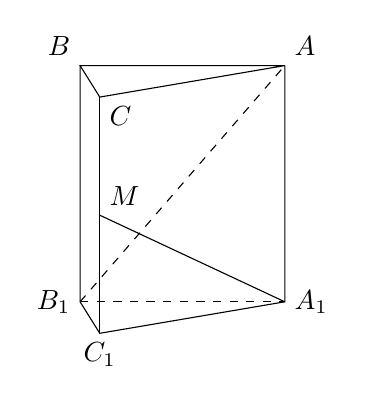
\begin{tikzpicture}[scale=1.0]
  \coordinate (B) at (0,3);
  \coordinate (A) at (2.6,3);
  \coordinate (C) at (0.25,2.6);
  \coordinate (B1) at (0,0);
  \coordinate (A1) at (2.6,0);
  \coordinate (C1) at (0.25,-0.4);
  \coordinate (M) at (0.25,1.1);
  \draw (B)--(A)--(C)--cycle;
  \draw (B)--(B1)--(C1)--(A1)--(A);
  \draw (C)--(C1);
  \draw (M)--(A1);
  \draw[dashed] (B1)--(A1);
  \draw[dashed] (B1)--(A);
  \node[above left] at (B) {$B$};
  \node[above right] at (A) {$A$};
  \node[below right] at (C) {$C$};
  \node[left] at (B1) {$B_1$};
  \node[right] at (A1) {$A_1$};
  \node[below] at (C1) {$C_1$};
  \node[above right] at (M) {$M$};
\end{tikzpicture}
